\chapter{Coordenadas curvilíneas}

\section{Coordenadas Cartesianas}
\noindent Posición:
\begin{eqnarray}
\vec{x} &=& x {\hat x} + y {\hat y} + z {\hat z}
\end{eqnarray}
Vector:
\begin{eqnarray}
\vec{A}
&=& A_x{\hat x} + A_y {\hat y} + A_z {\hat z}
\end{eqnarray}
Gradiente:
\begin{eqnarray}
 \vec\nabla\Psi&=&{\partial\Psi\over \partial x} {\hat x} + {\partial\Psi\over
\partial y} {\hat y}   + {\partial\Psi\over \partial z} {\hat z}
\end{eqnarray}
Divergencia
\begin{eqnarray}
 \vec\nabla \cdot \vec{A}
&=& \frac{\partial  A_x}{\partial x}+\frac{\partial  A_y}{\partial y}+\frac{\partial  A_z}{\partial z}
\end{eqnarray}
Rotor:
\begin{eqnarray}
\vec\nabla \times  \vec{A}
&=&   \left({\partial A_z \over \partial y} - {\partial A_y \over
\partial z}\right)  {\hat x}  +
   \left({\partial A_x \over \partial z} - {\partial A_z \over
\partial x}\right)  {\hat y}  +
   \left({\partial A_y \over \partial x} - {\partial A_x \over
\partial y}\right)  {\hat z}
\end{eqnarray}
Laplaciano
\begin{eqnarray}
 \nabla^2 \Psi
&=& {\partial^2\Psi\over \partial x^2} + {\partial^2\Psi\over \partial y^2} +
{\partial^2\Psi\over \partial z^2}
\end{eqnarray}
Desplazamiento:
\begin{eqnarray}
 d \vec{x} &=& dx {\hat x} + dy {\hat y} + dz {\hat z}
\end{eqnarray}
Elemento de superficie:
\begin{eqnarray}
 d \vec{S} &=& dy\,dz\, {\hat x} + dx\,dz\, {\hat y} +
dx\,dy\, {\hat z}
\end{eqnarray}
Elemento de volumen:
\begin{eqnarray}
 dV &=& dx\,dy\,dz
\end{eqnarray}


\section{Coordenadas Cilíndricas}
\begin{figure}[H]
    \centering
    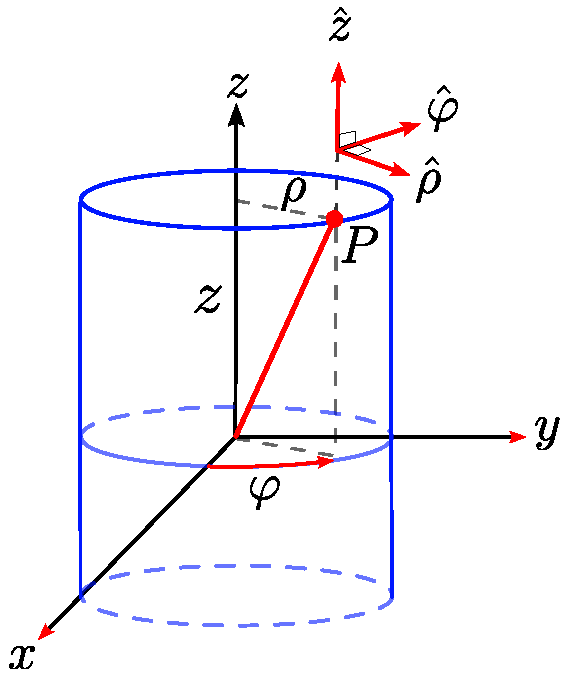
\includegraphics[scale = 0.6]{fig/Coordenadas-Cilindricas.pdf}
    \caption{Coordenadas cilíndricas $(\rho,\varphi, z)$ y sus vectores unitarios.}
    \label{fig:Coordenadas-Cilindricas}
\end{figure}

\noindent Definición:
\begin{equation}
    x  =  \rho\cos\varphi , \qquad
    y  =  \rho\sin\varphi , \qquad
    z =  z
\end{equation}
\begin{equation}
    \rho  =  \sqrt{x^2 + y^2} , \qquad
    \varphi  = \arctan{(y/x)}, \qquad
     z=  z
\end{equation}
Vectores unitarios:
\begin{align}
    \hat{\rho} &= %\frac{1}{\norm{\frac{\partial \Vec{x}}{\partial \rho}}}\frac{\partial \Vec{x}}{\partial \rho} =
    				 \cos \varphi \,\hat{x} + \sin \varphi \,\hat{y}, \\
    \hat{\varphi} &= %\frac{1}{\norm{\frac{\partial \Vec{x}}{\partial \varphi}}}\frac{\partial \Vec{x}}{\partial \varphi} = 
    				- \sin \varphi \,\hat{x} + \cos \varphi \, \hat{y},  \\
    \hat{z} &= %\frac{1}{\norm{\frac{\partial \Vec{x}}{\partial z}}}\frac{\partial \Vec{x}}{\partial z} = 
    			\hat{z} .
\end{align}
\begin{align}
    \hat{x} &= \cos \varphi \,\hat{\rho} - \sin \varphi \, \hat{\varphi}, \\
    \hat{y} &= \sin\varphi \, \hat{\rho} + \cos \varphi \,\hat{\varphi}.
\end{align}
Posición:
\begin{equation}
\vec{x} = \rho \hat{\rho} + z \hat{z}.
\end{equation}
Vector
\begin{equation}
\vec{A} =A_\rho {\hat \rho} + A_\varphi {\hat \varphi} +
A_z {\hat z}
\end{equation}
Gradiente:
\begin{eqnarray}
 \vec\nabla\Psi&=&{\partial\Psi\over \partial \rho} {\hat \rho}
  + {1 \over \rho}{\partial\Psi\over \partial \varphi} {\hat \varphi}
  + {\partial\Psi\over \partial z} {\hat z}
\end{eqnarray}
Divergencia
\begin{eqnarray}
 \vec\nabla \cdot \vec{A}
&=&  {1 \over \rho}{\partial \left( \rho A_\rho  \right) \over \partial
\rho}  + {1 \over \rho}{\partial A_\varphi \over \partial \varphi}
  + {\partial A_z \over \partial z}
\end{eqnarray}
Rotor:
\begin{eqnarray}
\vec\nabla \times  \vec{A}
&=&   \left({1 \over \rho}{\partial A_z \over \partial \varphi}
    - {\partial A_\varphi \over \partial z}\right)  {\hat \rho} +
\left({\partial A_\rho \over \partial z} - {\partial A_z \over
\partial \rho}\right)  {\hat \varphi} \nonumber\\
&&+  {1 \over \rho}\left({\partial \left( \rho A_\varphi \right) \over
\partial \rho}     - {\partial A_\rho \over \partial \varphi}\right) {\hat z}
\end{eqnarray}
Laplaciano
\begin{eqnarray}
 \nabla^2 \Psi
&=& {1 \over \rho}{\partial \over \partial \rho}\left(\rho {\partial\Psi\over
\partial \rho}\right)
  + {1 \over \rho^2}{\partial^2\Psi\over \partial \varphi^2}
  + {\partial^2\Psi\over \partial z^2} \\
\end{eqnarray}
Desplazamiento:
\begin{eqnarray}
 d \vec{x}
 &=& d\rho {\hat \rho} + \rho d\varphi {\hat \varphi} +dz {\hat z}
\end{eqnarray}
Elemento de superficie:
\begin{eqnarray}
 d \vec{S}
&=& \rho\, d\varphi\, dz\, {\hat \rho} + d\rho
\,dz\, {\hat \varphi} +  \rho \,d\rho\, d\varphi \, {\hat z}
\end{eqnarray}
Elemento de volumen:
\begin{eqnarray}
 dV
 &=& \rho\, d\rho\, d\varphi\, dz
\end{eqnarray}
\begin{figure}[H]
    \centering
    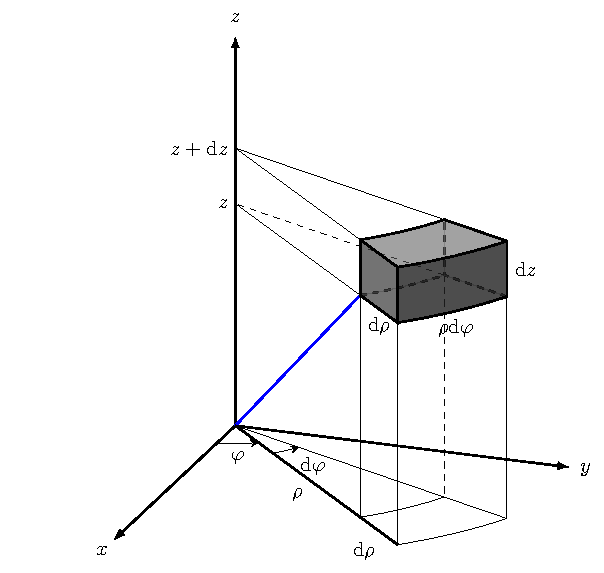
\includegraphics[scale=0.7]{fig/volumen-cilindricas.pdf}
    \caption{Elementos infinitesimales en coordenadas cilíndricas. Adaptado a partir de versión de A. Tsagkaropoulos, disponible en \href{https://tikz.net/cylindrical_volume/}{esta página}.}
    \label{fig:Vol-Cilindricas}
\end{figure}
\section{Coordenadas Esféricas}
\begin{figure}[H]
    \centering
    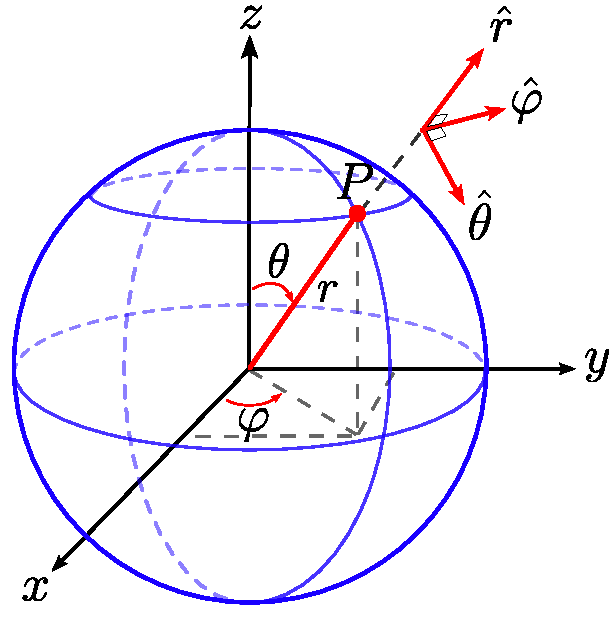
\includegraphics[scale = 0.5]{fig/Coordenadas-Esfericas.pdf}
    \caption{Coordenadas esféricas $(r,\theta,\varphi)$ en conjunto con sus vectores unitarios.}
    \label{fig:Coordenadas-Esfericas}
\end{figure}
\noindent Definición:
\begin{equation}
    x  =  r\sin\theta\cos\varphi, \qquad
    y  =  r\sin\theta\sin\varphi , \qquad
    z  =  r\cos\theta
\end{equation}
\begin{equation}
    r  =  \sqrt{x^2 + y^2 + z^2} , \quad
    \theta  =  \arccos(\frac{z}{r}) = \arctan{\frac{\sqrt{x^2+y^2}}{z}}, \quad
    \varphi  =  \arctan{(y/x)}
\end{equation}
Vectores unitarios:
\begin{align}
    \hat{r} &= %\frac{1}{\norm{\frac{\partial \Vec{x}}{\partial r}}}\frac{\partial \Vec{x}}{\partial r} 
    			\sin \theta \cos \varphi \,\hat{x} + \sin \theta \sin \varphi \,\hat{y} + \cos \theta \,\hat{z}, \label{rxyz} \\
    \hat{\theta} &= %\frac{1}{\norm{\frac{\partial \Vec{x}}{\partial \theta}}}\frac{\partial \Vec{x}}{\partial \theta} 
    			\cos \theta \cos \varphi \,\hat{x} + \cos \theta \sin \varphi \,\hat{y} - \sin \theta   \,\hat{z},  \\
    \hat{\varphi} &= %\frac{1}{\norm{\frac{\partial \Vec{x}}{\partial \varphi}}}\frac{\partial \Vec{x}}{\partial \varphi} 
    			- \sin \varphi \,\hat{x} + \cos \varphi \,\hat{y} . \label{varphixyz}
\end{align}
\begin{align}
    \hat{x} &= \sin \theta \cos \varphi \,\hat{r} + \cos \theta \cos \varphi \,\hat{\theta} - \sin \varphi \,\hat{\varphi},\\
    \hat{y} &= \sin \theta \sin\varphi \,\hat{r} + \cos \theta \sin \varphi \,\hat{\theta} + \cos \varphi \,\hat{\varphi}, \\
    \hat{z} &= \cos \theta \,\hat{r} - \sin \theta \,\hat{\theta}.
\end{align}
Posición:
\begin{equation}
\vec{x} = r \hat{r}
\end{equation}
Vector:
\begin{eqnarray}
\vec{A}
&=& A_r {\hat r} + A_\theta {\hat \theta} +
A_\varphi {\hat \varphi}
\end{eqnarray}
Gradiente:
\begin{eqnarray}
 \vec\nabla\Psi
 &=& {\partial\Psi\over \partial r} {\hat r}
  + {1 \over r}{\partial\Psi\over \partial \theta} {\hat \theta}
  + {1 \over r\sin\theta}{\partial\Psi\over \partial \varphi} {\hat \varphi}
\end{eqnarray}
Divergencia
\begin{eqnarray}
 \vec\nabla \cdot \vec{A}
&=& {1 \over r^2}{\partial \left( r^2 A_r \right) \over \partial r}
  + {1 \over r\sin\theta}{\partial \over \partial \theta} \left(
A_\theta\sin\theta \right)
  + {1 \over r\sin\theta}{\partial A_\varphi \over \partial \varphi}
\end{eqnarray}
Rotor:
\begin{eqnarray}
\vec\nabla \times  \vec{A}
&=&  {1 \over r\sin\theta}\left({\partial \over \partial \theta}
\left( A_\varphi\sin\theta \right)    - {\partial A_\theta \over \partial
\varphi}\right) {\hat r} \nonumber\\
&&+    {1 \over r}\left({1 \over \sin\theta}{\partial A_r \over \partial
\varphi} - {\partial \over \partial r} \left( r A_\varphi \right) \right)
 {\hat \theta}  +   {1 \over r}\left({\partial \over \partial r} \left( r
A_\theta
\right)  - {\partial A_r \over \partial \theta}\right)  {\hat \varphi}
\end{eqnarray}
Laplaciano
\begin{eqnarray}
 \nabla^2 \Psi
&=&  {1 \over r^2}{\partial \over \partial r}\left(r^2 {\partial\Psi\over
\partial r}\right)   + {1 \over r^2\sin\theta}{\partial \over \partial
\theta}\left(\sin\theta {\partial\Psi\over \partial \theta}\right)
  + {1 \over r^2\sin^2\theta}{\partial^2\Psi\over \partial \varphi^2}
\end{eqnarray}
Desplazamiento:
\begin{eqnarray}
 d \vec{x}
&= & dr {\hat r} + rd\theta {\hat \theta} +r\sin\theta d\varphi {\hat \varphi}
\end{eqnarray}
Elemento de superficie:
\begin{eqnarray}
 d \vec{S}
&=& r^2 \sin\theta \,d\theta \,d\varphi \, {\hat r} + r\sin\theta
\,dr\,d\varphi \, {\hat \theta} +  r\,dr\,d\theta\, {\hat \varphi}
\end{eqnarray}
Elemento de volumen:
\begin{eqnarray}
 dV
&=& r^2\sin\theta \,dr\,d\theta\, d\varphi
\end{eqnarray}
\begin{figure}[H]
    \centering
    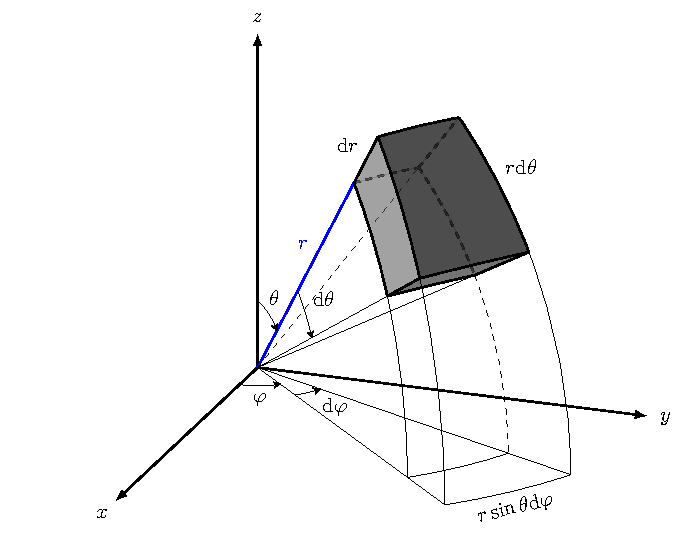
\includegraphics[scale=0.7]{fig/volumen-esfericas.pdf}
    \caption{Elementos infinitesimales en coordenadas esféricas. Adaptado a partir de versión de A. Tsagkaropoulos, disponible en \href{https://tikz.net/spherical_volume/}{esta página}.}
    \label{fig:Vol-Esfericas}
\end{figure}